\part{Preliminaries}
\chapter{Introduction, one-dimensional systems}
In this course, you are going to learn a lot about mathematical modelling.
The first half of the course is concerned with filling in some of the
important gaps in your mathematical toolkit.  

We are going to largely restrict ourselves to modelling using Ordinary
Differential Equations (ODEs). We can learn how maths can be applied
effectively in a great many different scenarios using ODEs, and plus you
already have some prior exposure to these, so it's not all new! 

Now, probably your experience of differential equations has been largely
constrained to finding analytical solutions to them - given a problem,
you've searched for an appropriate method to solve it, perhaps separation
of variables or something more exotic, and then used all of the provided
information about your problem to come up with a solution. This is but one
of three approaches that we will use for differential equations, and the
one that we will use the least! The other two are 
\begin{itemize}
    \item Graphical methods
    \item Numerical methods
\end{itemize}
The emphasis in this course is on the qualitative behaviour of dynamical
systems, which for us will mean systems governed by differential or
difference equations. We are not so much concerned about specific
solutions, but rather how the system behaves for different choices of
parameters or initial conditions.

We will learn how to use \emph{phase portraits} and \emph{bifurcation
diagrams}, special pictures that illustrate the dynamics of systems to
interpret their behaviour, and we'll usually be using numerical methods to
simulate our differential equations, as the types of equations encountered
during modelling are rarely solvable analytically.

We don't have a particular textbook for this course, but the development of
the material from the first section is based on the presentation in
\emph{Nonlinear Dynamics and Chaos} by Stephen Strogatz.

\section{General systems}
We are going to be concerned with systems of differential equations of the
form 
\begin{equation}
    \begin{split}
        \dot{x_1} &= f_1(x_1, \ldots, x_n) \\
        &\vdots \\
        \dot{x_n} &= f_n(x_1, \ldots, x_n)
    \end{split}
\end{equation}
The overdots signify differentiation with respect to time $t$. These
systems are known as systems of \emph{autonomous} differential equations,
as there is no $t$ dependence in their right hand sides. Higher order
differential equations, such as 
\begin{equation*}
    \ddot{x} + a\dot{x} + x = 0
\end{equation*}
can readily be put into this format by the standard trick of defining the
variables $x_1 = x$, $x_2 = \dot{x}$. We then have the system
\begin{equation*}
    \begin{split}
        \dot{x_1} &= x_2 \\
        \dot{x_2} &= -x_1 - ax_2.
    \end{split}
\end{equation*}
We just define our $x_i$ to be the $(i-1)$-th derivative of $x$,
stopping one before we get to the highest order derivative present.

\section{One-dimensional systems}
Right. Let's start with the simplest case, just one differential equation
in one variable,
\begin{equation*}
    \dot{x} = f(x).
\end{equation*}
In fact, let's start with a specific example,
\begin{equation*}
    \dot{x} = \sin x.
\end{equation*}
We are going to try to analyse this by developing some graphical methods,
rather than relying on being able to solve it. Which, by the way, we could
if we wanted to -- this happens to be a differential equation that
\emph{does} have a closed-form solution. OK, let's do that real quick, just
to remember how painful and tedious an exercise this is. We start by
separating variables
\begin{equation*}
    \frac{1}{\sin x}\frac{dx}{dt} = 1
\end{equation*}
which gives
\begin{equation*}
    t = \int \csc x \, dx = \ln \abs{\csc x + \cot x} + C.
\end{equation*}
Putting in an initial condition $x(0) = x_0$ gives
\begin{equation*}
    t = \ln \abs{\frac{\csc{x_0} + \cot x_0}{\csc x + \cot x}}
\end{equation*}
Say something about that without getting a headache, I dare you. Can you
tell me
\begin{enumerate}
    \item With $x_0 = 1$, describe what happens to the solution as $t \to
        \infty$.
    \item What happens to $x$ as $t \to \infty$ for an arbitrary initial
        condition $x_0$?
\end{enumerate}
This kind of qualitative information is very difficult to glean from this
closed-form solution. We need a better way.

\section{A geometrical approach}
Let's now imagine that our equation $\dot{x} = \sin x$ represents the
velocity of a particle on the $x$ axis. The differential equation $\dot x =
\sin x $ represents a \emph{vector field} on the line, it specifies the
velocity vector $\dot x$ at each point $x$. 

When our particle is at position
$x_0$, it has velocity $f(x_0)$, and if that's positive, it means it's
going to zoom off in the positive $x$ direction, or, if it's negative, it
will head left. We can draw this in Fig.~\ref{fig:sinflow} by indicating
with an arrow which way the flow is moving, and a dot where $f(x) = 0$,
indicating that our particle is stationary. These points where $\dot x = 0$
are called \emph{fixed points}.  The fixed points marked with black dots
are \emph{stable fixed points} or \emph{attractors}, as flows are attracted
to them, and the fixed points marked as white dots are \emph{unstable fixed
points} or \emph{repellors}, as a small perturbation from the fixed point
will cause the particle to move away from it.

We can trace the path that our particle takes on our diagram, this is
called a \emph{trajectory}. The diagram in Fig.~\ref{fig:sinflow} is called
a \emph{phase portrait}.

\begin{figure}[h!]
  \centering
  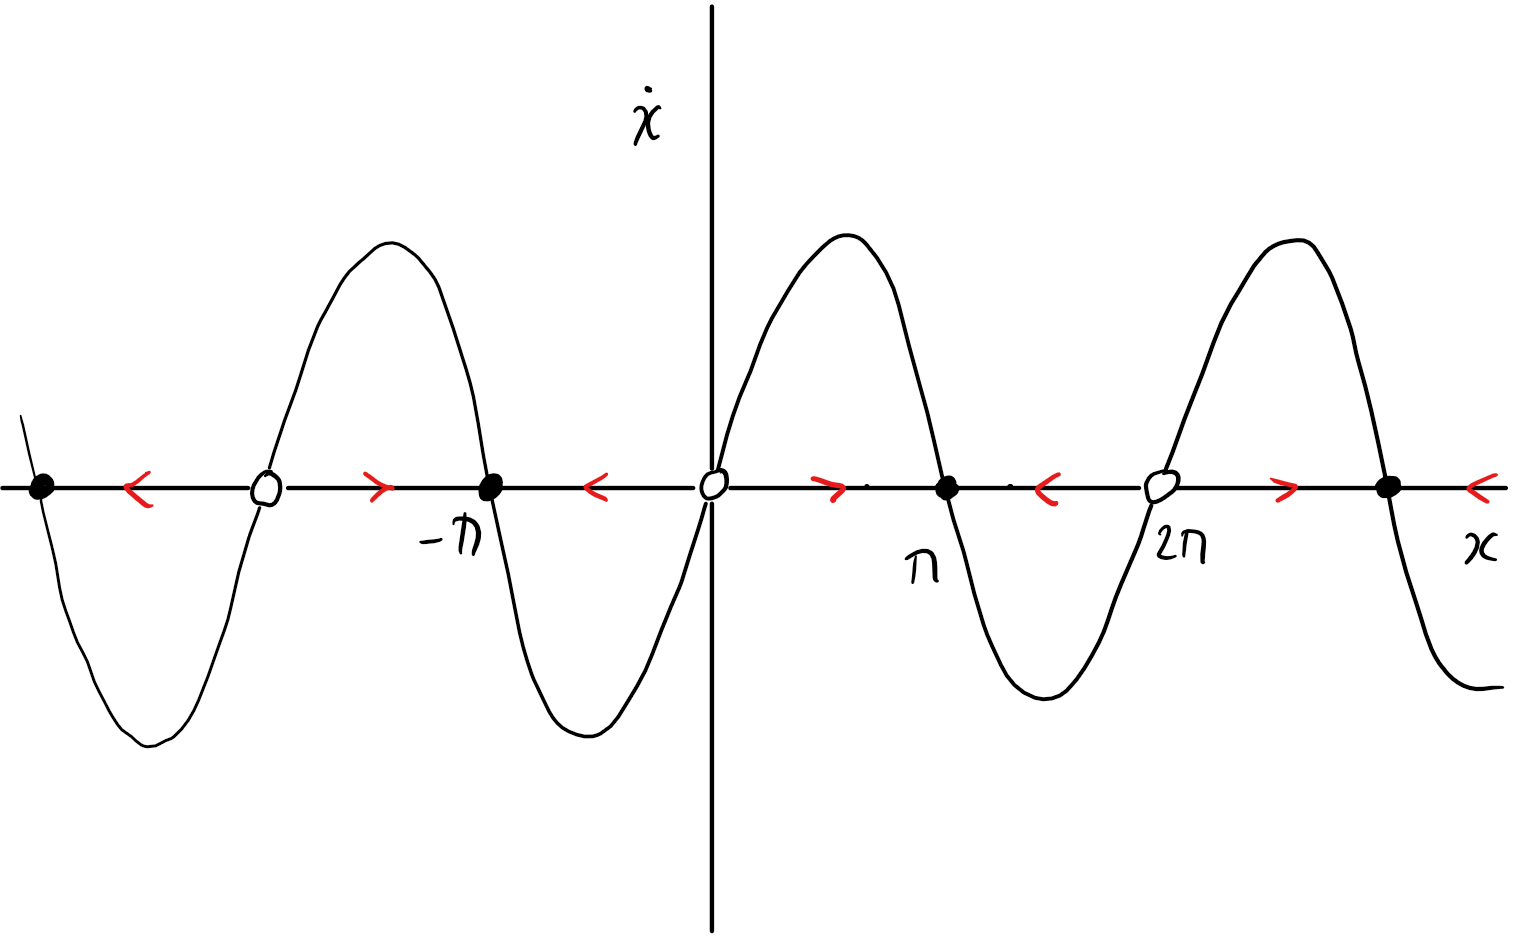
\includegraphics[width=\linewidth]{figs/sinflow}
  \caption{Phase portrait for $\dot x = \sin x$.}
  \label{fig:sinflow}
\end{figure}

We can now produce a pretty good qualitative sketch of what happens from an
initial condition of $x_0 = 1$. This is just to the left of $\pi/2$, and so
the particle will be moving right, and accelerating initially. As it
crosses $\pi/2$, the velocity $\dot x$ will start to decrease, and the
particle will eventually come to a halt when it reaches $\pi$. So the
solution plotted as $x$ vs $t$ will look something like:

\begin{center}
    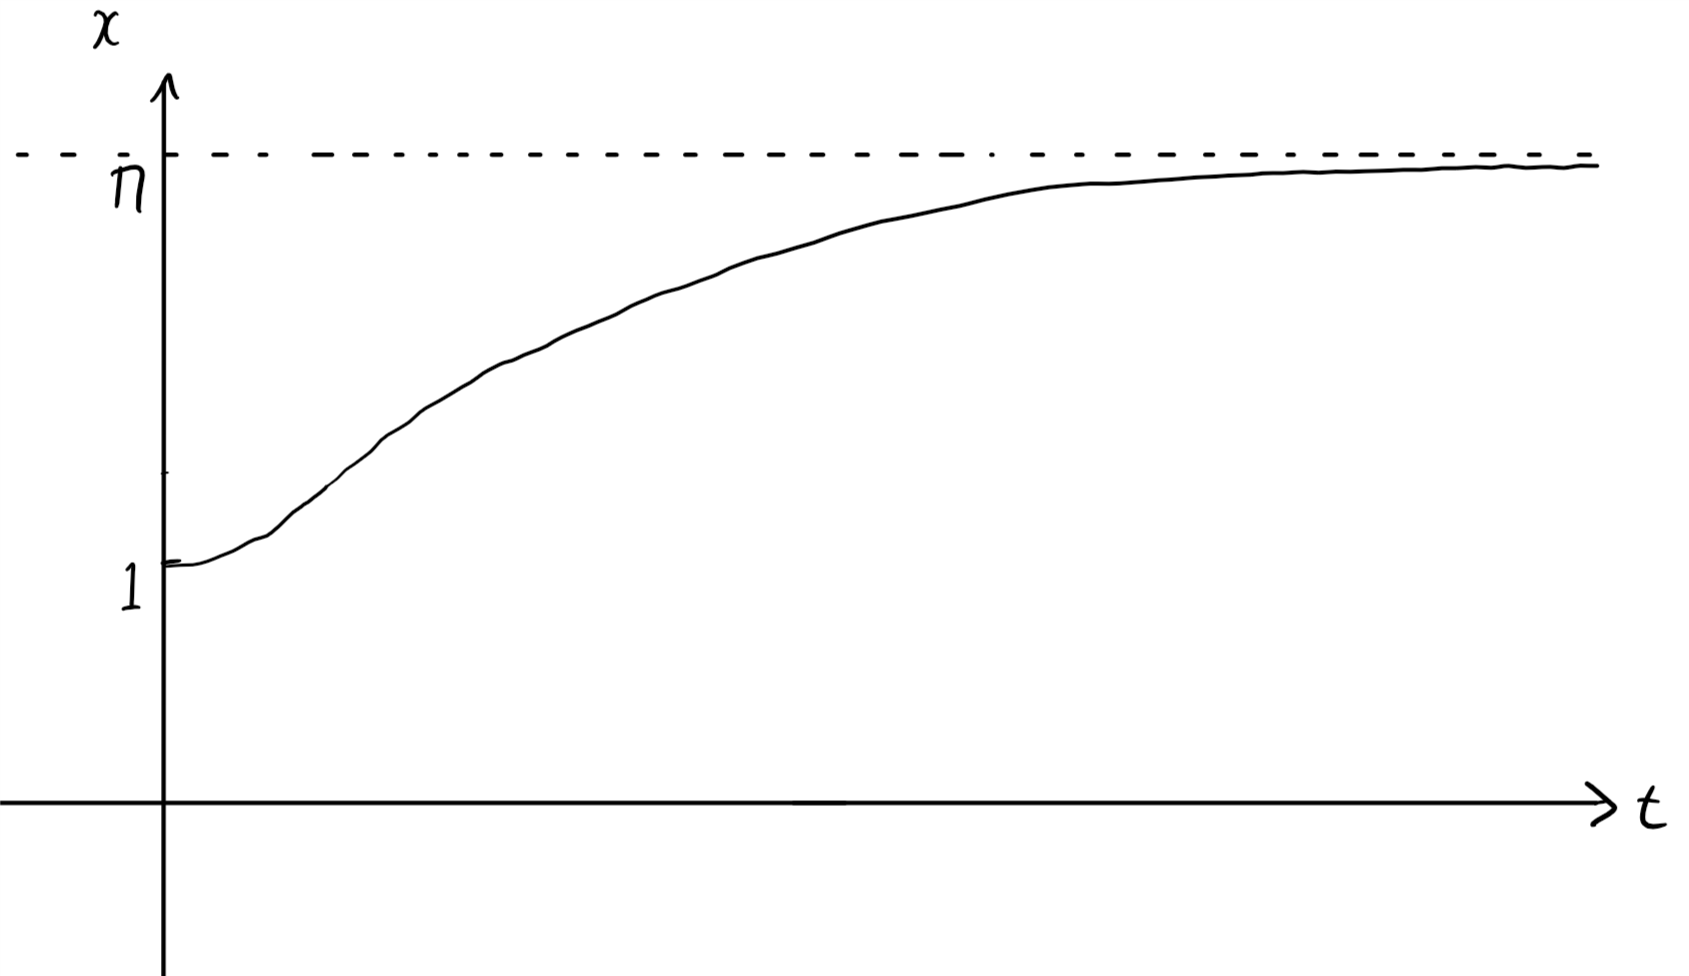
\includegraphics[width=\linewidth]{figs/sintrajectory}
\end{center}

You can see the curve is initially concave up, then concave down when it
crosses $\pi/2$, and eventually slows up and approaches $\pi$. Our sketch
doesn't tell us anything about how long this takes, but it gives us a good
qualitative idea of what's happening. We could do this exercise for any
initial condition.

\begin{example}
    Find all fixed points for $\dot x = x^2 - 1$, and classify their
    stability.
\end{example}

\begin{example}
    Sketch the phase portrait corresponding to $\dot x = x - \cos x$ and
    determine the stability of all of the fixed points.
\end{example}

\chapter{Population modelling, linear stability}
\section{Population growth}
One area of modelling that we can dive into straight away, is that of
population growth. The simplest model of the growth of a population of
organisms is $\dot N = rN$, where $N(t)$ is the population at time $t$, and
$r > 0$ is the growth rate. Now, this is a very simplistic model, in that
it treats population as a continuous variable, and assumes that the number
of births in any given time period is proportional to the population
itself. This is not altogether unreasonable, and does in fact describe the
early stage of growth of some populations fairly well. 

This model is readily solved analytically to give $N(t) = N_0 e^{rt}$ (you
should train yourself to know this result automatically). So the model
predicts exponential growth indefinitely. Which clearly is not practical.
A useful concept is that of a \emph{carrying capacity}, i.e. a population
level above which the growth rate is negative, indicating that the
resources available are not sufficient to sustain a greater population.
Biologists often model the population growth rate as a decreasing function
of population, which starts of at $r$ when the population is small, but
then crosses zero when the population hits the carrying capacity $K$, as
shown in Fig~\ref{fig:carryingcapacity}.

\begin{figure}[h]
  \centering
  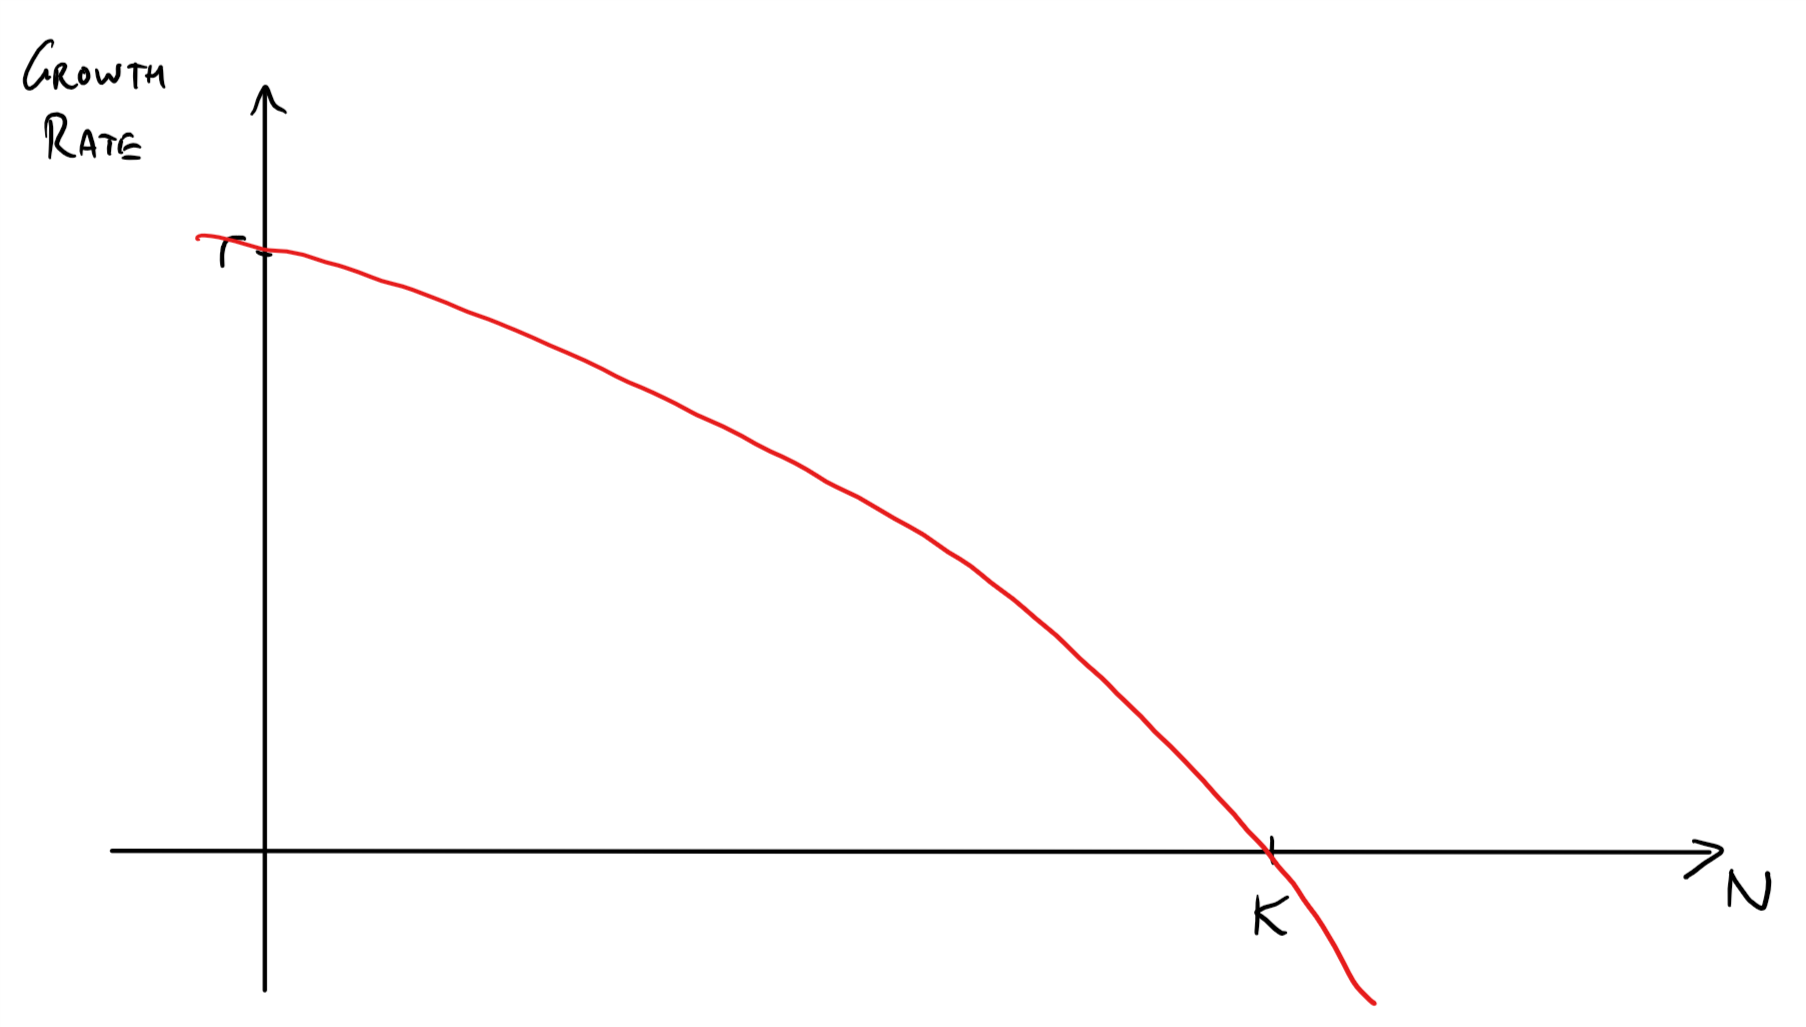
\includegraphics[width=\linewidth]{figs/carryingcapacity}
  \caption{}
  \label{fig:carryingcapacity}
\end{figure}

The simplest such model, just has a linearly decreasing growth rate from
$r$ to $0$, as shown in Fig~\ref{fig:logisticgrowth}. The corresponding
model, known as the \emph{logistic equation} is simply
\begin{equation}\label{eq:logistic}
    \dot N = rN \left(1 - \frac{N}{K}\right).
\end{equation}
\begin{figure}[h]
  \centering
  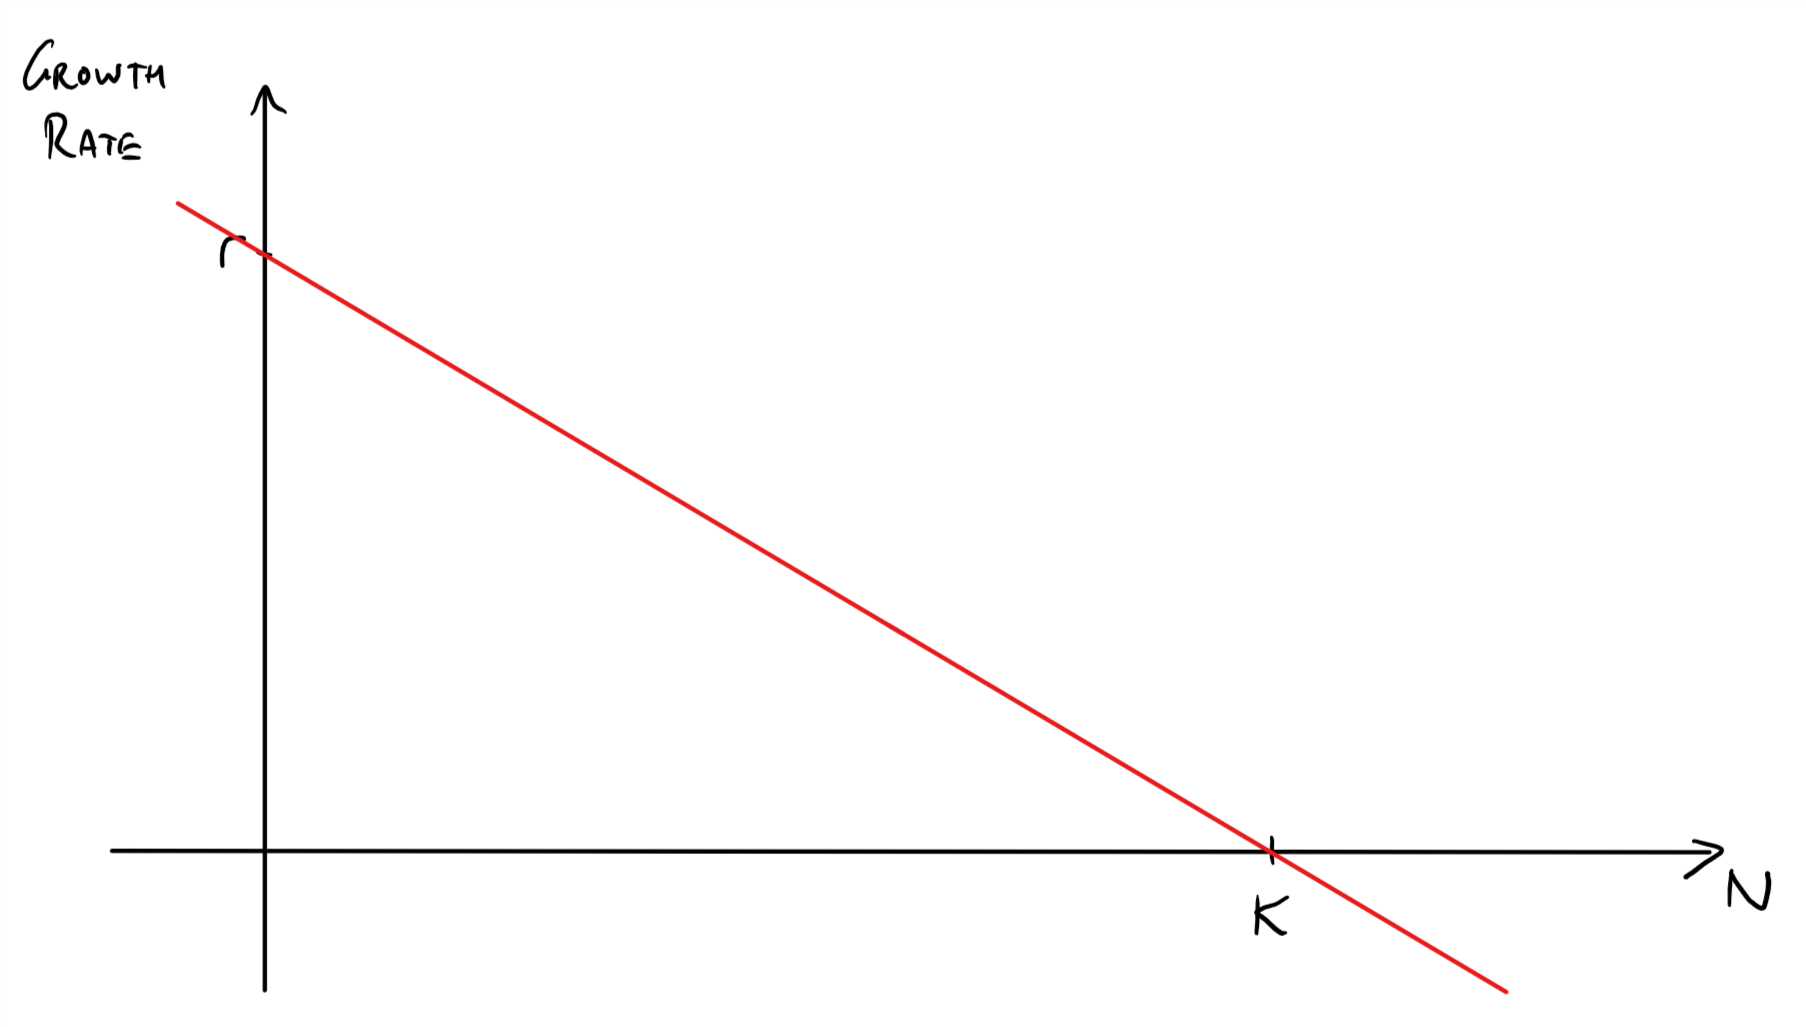
\includegraphics[width=\linewidth]{figs/logisticgrowth}
  \caption{Logistic growth rate}
  \label{fig:logisticgrowth}
\end{figure}

\begin{example}
    Draw a phase portrait of the logistic equation, find and classify the
    stability of all of the fixed points, and draw some qualitatively
    correct solutions of the system for representative initial conditions.
\end{example}

\section{Linear Stability Analysis}
So far we've just relied on looking at our pictures to determine the
stability of fixed points. It'd be good if we could do it mathematically,
and even better if we could get some indication of how quickly trajectories
either diverged from, or converged to, our fixed points.

We can get this information by \emph{linearising} our model around the
fixed point. This means replacing it with a linear approximation of the
nonlinear equation. We know that linear equations ($\dot x = a x$), give
exponential solutions, and we know characteristic timescales of exponential
behaviour.

Let $x^\star$ be a fixed point, and let $\eta(t) = x(t) - x^\star$ be a
small perturbation from $x^\star$. We'd like to see whether our
perturbation grows or decays, so we derive a differential equation for
$\dot \eta$,
\begin{equation*}
    \dot \eta = \frac{d}{dt} (x - x^\star) = \dot x = f(x^\star + \eta).
\end{equation*}
We can then expand $f$ in a Taylor expansion around $x^\star$, giving
\begin{equation*}
    f(x^\star + \eta) = f(x^\star) + f'(x^\star) \eta +
    \mathcal{O}(\eta^2),
\end{equation*}
where $\mathcal{O}(\eta^2)$ denotes terms that are dominated by a quadratic
as $\eta$ approaches $0$. Thus
\begin{equation*}
    \dot \eta = f'(x^\star)\eta + \mathcal{O}(\eta^2).
\end{equation*}
If $f'(x^\star) \neq 0$, then the $\mathcal{O}(\eta^2)$ are negligible near
$\eta = 0$, and we can approximate the equation as
\begin{equation*}
    \dot \eta \approx f'(x^\star) \eta.
\end{equation*}
This is called the \emph{linearisation} about $x^\star$. This shows that
perturbations from the fixed point grow exponentially if $f'(x^\star) > 0$,
and decay exponentially if $f'(x^\star) < 0$. If $f(x^\star) = 0$, it means
that our assumption that the $\mathcal{O}(\eta^2)$ terms that we neglected
are not in fact negligible, and we need to determine the stability some
other way (using graphical methods for example).

The linearisation also gives us a \emph{characteristic} time scale for the
equation near the steady state, the time $1/\abs{f'(x^\star)}$ is the time
for $x(t)$ to vary significantly near $x^\star$.

\begin{example} Use linear stability analysis to classify the fixed points
    of the equation from last lecture, $\dot x = \sin x$.
\end{example}

\begin{example} Classify the fixed points of the logistic equation, and
    find the characteristic time scale in each case.
\end{example}

\section{Existence and Uniqueness}
We've been assuming that solutions to our differential equations exist
without really taking all that much care. Consider the following equation
\begin{equation*}
    \dot x = x^{1/3}, \qquad x(0) = 0.
\end{equation*}

Clearly $x = 0$ is a fixed point, so $x(t) = 0$ is a valid solution to our
equation. But, if we try solve it, separating variables we get
\begin{equation*}
    \int x^{-1/3}\,dx = \int\,dt
\end{equation*}
which gives
\begin{equation*}
    \frac{3}{2} x^{2/3} = t + C
\end{equation*}
Our initial condition gives $C = 0$, and so the solution is
\begin{equation*}
    x(t) = \left(\frac{2t}{3} \right)^{3/2}.
\end{equation*}
But, wait - we already have a solution $x = 0$. How can there be two? Turns
out the problem is the first derivative at $0$. If we draw a phase
portrait, we see that $f'(0)$ is in fact infinite, and this is enough to
break the uniqueness of our system. So, we need some restrictions to ensure
that we actually have a unique solution to our system. In particular
\begin{existenceuniqueness}
    Consider the initial value problem $\dot{x} = f(x)$, $x(0) = x_0$.
    Suppose that $f(x)$ and $f'(x)$ are continuous on an open interval $R$
    of the $x$-axis, and suppose that $x_0$ is a point on $R$. The the
    initial value problem has a unique solution $x(t)$ on some interval
    $(-\tau, \tau)$ about $t = 0$.
\end{existenceuniqueness}



